% Chapter 4
\chapter{Multiplier Analysis}
\label{Chapter4}

\begin{doublespacing}

\section{Introduction}
\label{sec:4.1}

Input-Output (IO) multipliers are used widely in order to simulate shocks to an economy. The notion of multiplier modeling rests on the assumption that there is an output response first to meet the demand shock. Second, there are other observable changes in the economy's output and these are assumed to be the multipliers (see Section \ref{sec4.3} for a more detailed treatment of these changes) \cite{Miller2009}. Multipliers are thus used to measure how a exogenous change to the model affects the economy \cite{Miller2009}.

\bigskip

Most commonly demand shocks are modelled using IO Type I and Type II multipliers. However, there several methods are used to derive these multipliers. This paper analyses common methods of Type II output multipliers for the Scottish economy Note that the findings of this paper are transferable to the discussion of other types of multipliers, e.g. income or employment multipliers.The aim is to establish which method offers the best fit for multiplier modelling. Four methods are used for this study. Two of these methods use pure IO data and can be computed with the data available in an IO dataset alone. The other two methods use more comprehensive data for the endogenising of the Household sector.

\bigskip

In order to determine the best fitting Type II output multiplier for the Scottish economy, the methods presented in this paper need to be compared to a standard. The most appropriate benchmark for testing the fit of the Type II multipliers is assumed to be the SAM output multiplier. The 2009 Scottish SAM \shortcite{SCOSAM} offers the most complete dataset for the Scottish economy for that year. The output multiplier derived from that dataset therefore provides the best fit for multiplier modelling. Thus, if a Type II output multiplier is to be used and not a SAM output multiplier it is advisable to chose the best fitting Type II benchmarked against the SAM multiplier.

\bigskip

The Type I, the Type II and the SAM output multiplier are extensions of each other. All use an IO Table as the main dataset for the derivation of the multipliers. The data used in this paper are derived from the 2009 Scottish Industry-by-Industry (IxI) IO Tables and the 2009 Scottish SAM \shortcite{SCOSAM} as well as from the Scottish National Accounts Project (SNAP) \cite{ScotGov2013c}.

\bigskip

This paper is structured as follows. The second Section describes the data used for the calculation of the Type I, the Type II and the SAM multipliers. The third Section outlines the computation and interpretation of the Type I, the Type II and the SAM multipliers. The fourth Section outlines four common methods used for the derivation of Type II output multipliers for the Scottish economy. The fifth Section analyses the derived multipliers and the sixth Section concludes.

\newpage

%%%%%%%%%%%%%%%%%%%%%%%%%%%%%%%%%%%%%%%%%%%%%%%%%%%%%%%%%%
%SECTION
%%%%%%%%%%%%%%%%%%%%%%%%%%%%%%%%%%%%%%%%%%%%%%%%%%%%%%%%%%

\section{Data}
\label{sec:4.2}

The main data source for the Type I, the Type II and the SAM output multiplier in this paper are the 2009 Scottish IxI Tables \cite{ScottishGovernment2013a}. Secondly, the 2009 Scottish SAM is used both for the computation of one of the Type II methods studied in this paper (see Section \ref{sec:4.4.3}) as well as for the derivation of the SAM output multiplier (see Section \ref{sec:4.3.3}). Lastly the figure for ``Total household income from all sources'' from SNAP is used for endogenising the Household sector in one of the methods discussed in this paper (see Section \ref{sec:4.4.4}). This section presents the data sources outlined above in the same order below.

\subsection{2009 Scottish IxI Tables}
\label{sec:4.2.1}

Input-Output (IO) Tables provide a snapshot of an economy for a given year. They present macro-economic aggregates and their sectoral disaggregation. IO Tables show payments to factors of production (wages and OVA) as well as information on institutional accounts (i.e. households, government and corporations). The IxI Tables used here are for the calendar year 2009 and they are also the basis for the 2009 Scottish SAM (see Section \ref{sec:4.2.2}). The IxI Tables show the destination of industry output, for example primary manufacturing products. The columns of the IxI Table show purchases made by industries and final demand from each Scottish industry's output arising from both principal production and intermediate demand. Conversely, the rows provide a breakdown of industry receipts by origin.

\bigskip

The data contained in the IxI Tables enables the computation of Type I output multipliers (see Section \ref{sec:4.3.1}). Further, the data in these IO Tables is sufficient to calculate two of the Type II multiplier methods discussed below (see Section \ref{sec:4.4.1} and \ref{sec:4.4.2}). Note that the data contained in the 2009 Scottish IxI Tables is for mainland activities only. Thus the multiplier analysis below is restricted to that geographic area of economic activity in Scotland.

\subsection{2009 Scottish SAM}
\label{sec:4.2.2}

The SAM can be considered as extended IO Tables. As well as the information outlined above (see Section \ref{sec:4.2.1}), a SAM also records the distribution and redistribution of income. The focus of a SAM therefore lies in recording interrelationships at the meso-level with emphasis on distributive aspects \cite{Keuning1988a}. It is concerned with the systematic organisation of information about the economic and social structure of a country, region, or city, in a particular time period - usually a year \cite{King1981a}.  

\bigskip

In contrast to IO tables, the SAM records flows from producing sectors to factors of production and then on to institutional accounts and finally back to the demand for goods \cite{Adelman1986a}. That is, IO tables show payments to factors of production (wages and OVA) but do not show subsequent flows to institutions. As such, a SAM is different from an IO table in that it contains complete information on institutional accounts (i.e. households, government and corporations), instead of solely tracing income and expenditure flows associated with the production of commodities \shortcite{Breisinger2010a}.

\bigskip

This paper makes the assumption that the comprehensive information contained in a SAM provides the basis for robust output multiplier computations. Therefore, the 2009 Scottish SAM is used to construct SAM output multipliers, which are used as benchmarks for the analysis of the methods discussed in Section \ref{sec:4.1}.

\subsection{SNAP}
\label{sec:4.2.3}

SNAP is a quarterly publication by the Scottish Government aimed at offering a single data source on broad economic indicators. Currently it provides data on, inter alia, measures of GDP and Gross Disposable Household Income. The latter is of interest to this paper as it provides the ``Total household income from all sources'' used for the endogenising of the Household sector for one of the methods presented below (see Section \ref{sec:4.4}).

%%%%%%%%%%%%%%%%%%%%%%%%%%%%%%%%%%%%%%%%%%%%%%%%%%%%%%%%%%
%SECTION
%%%%%%%%%%%%%%%%%%%%%%%%%%%%%%%%%%%%%%%%%%%%%%%%%%%%%%%%%%

\newpage
    \section{Output Multiplier}
\label{sec:4.3}

IO Tables and SAMs allow for the computation for various types of multipliers, including income, employment and output multipliers. The focus here is on the latter. This is because, first, the output multiplier is calculated most directly. Second, it enables an extension of the discussion to other types of multipliers and their derivations. For example, different Type II computations of the income and of the employment multiplier can be analysed following the framework presented in this paper.

\bigskip

Three types of output multipliers are described below, starting with the simplest case the Type I. Next, the Type II output multiplier is outlined, which is the structure of the different kind of multipliers discussed in Section \ref{sec:4.4}. Last, the SAM output multiplier is discussed, which is the benchmark multiplier used for the analysis in Section \ref{sec:4.5}.

\subsection{Type I Output Multiplier}
\label{sec:4.3.1}

The Type I output multiplier also known as the simple output multiplier enables the estimation of knock-on effects throughout the Scottish economy of a change in final demand \cite{Miller2009}. The data used for this multiplier are the inter-industry linkages in the IxI Tables. That is the matrix made up of only the rows and columns of the Interindustry flows (see Figure \ref{fig:4.3.1} below) \footnote{ Note, the IxI and SAM Tables used for the multiplier calculations omit industries 7 (Oil \& gas extraction, metal ores) as well as 20 (Tobacco) as there are no data entries for either industry in the 2009 Scottish IxI Tables. Thus the total number of industries used here is 102, rather than the full 104 industries (under SIC 2007 code).}.

\subsubsection{Calculation}

The first step in deriving Input-Output (IO) multipliers is to construct the technical coefficient matrix, also referred to as the A-matrix. This matrix is calculated by dividing each entry of the inter-industry flows of the IO Tables by the relevant column total, i.e. the total expenditure in each sector \cite{Miller2009}. Following the calculation outlined below, the Leontief Inverse is calculated. The column-sums of which are the output multiplier for each sector (see Figure \ref{fig:4.3.1} ).

\bigskip

\begin{figure}[hb]
\label{fig:4.3.1}
  \centering
  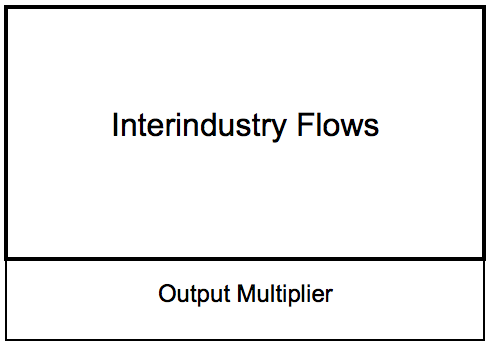
\includegraphics[width=3in]{T1OutputMultiplier}
  \caption{Type I Output Multiplier}
\end{figure}

\bigskip

Below is a brief outline of how the $\textit{A}$-matrix of technical coefficients and the Leontief Inverse is derived. Note that the derivation of the a-coefficients is the same for the different types of multipliers discussed in this section as well as for the types in Section \ref{sec:4.4}.

\bigskip

First, the individual column entries of the inter-industry flows from the IO Tables are divided by the relevant column total. For example, the first sector in the 2009 Scottish IxI Tables is Agriculture \cite{ScottishGovernment2013a}. The figure for the inter-industry flow from Agriculture to Agriculture is \textsterling339m and the column total (``Total output at basic prices'') for Agriculture is \textsterling2,584.3m. This results in the technical coefficient being estimated at 0.131 (this figure corresponds to the $a_{11}$ in Equation \ref{eq:4.3.1}). Note that the $\textit{A}$-matrix below is also labelled as $A_{II}$. The capital i's here are for the industry-by-industry coefficients.

  \bigskip
\begin{singlespacing}
 \begin{equation} \label{eq:4.3.1}
  A = \begin{pmatrix}
  a_{1,1} & \cdots & a_{1,j} \\
  \vdots & \ddots & \vdots  \\
  a_{i,1} & \cdots & a_{i,j}
  \end{pmatrix} \end{equation} 
  \end{singlespacing} \bigskip

The next step in order to be able to calculate the Leontief Inverse, is to construct the $I-\textit{A}$-matrix (see Equation \ref{eq:4.3.4}). This matrix simply uses an identity matrix (see Equation \ref{eq:4.3.2}) and subtracts the $\textit{A}$-matrix (Equation \ref{eq:4.3.1}) from it. The resultant matrix from this calculation has positive values on the diagonal (i.e. the inter-industry flow entries for the individual sectors between themselves). All other entries are negative. Following the example above, the identity matrix gives the value 1 for the Agriculture-Agriculture entry. This is then subtracted by the technical coefficient $a_{11}$  at 0.131. The $(I-A)$-matrix entry (corresponding to $1-a_{11}$ in Equation \ref{eq:4.3.4}) is calculated at 0.869.

  \bigskip \begin{singlespacing} \begin{equation} \label{eq:4.3.2}
  I = \begin{pmatrix}
    1 & \cdots & 0 \\
    \vdots & \ddots & \vdots  \\
    0 & \cdots & 1
  \end{pmatrix} \end{equation} \end{singlespacing} 

  \begin{singlespacing} \begin{equation} \label{eq:4.3.3}
  I-A = \begin{pmatrix}
  1-a_{1,1} & \cdots & 0-a_{1,j} \\
  \vdots & \ddots & \vdots  \\
  0-a_{i,1} & \cdots & 1-a_{i,j}
   \end{pmatrix}   \end{equation} \end{singlespacing}  \bigskip

The last step for the calculation of the Leontief Inverse is inverting the I-A-matrix, thus deriving  $L=(I-A)^{(-1)}$ (see Equation \ref{eq:4.3.4}). The value for the Agriculture-Agriculture entry for the Leontief Inverse is calculated at 1.156 for the Type I output multiplier.

  \bigskip   \begin{singlespacing}  \begin{equation} \label{eq:4.3.4}
  L=(I-A)^{-1} = Inverse  \begin{pmatrix}
    1-a_{1,1} & \cdots & 0-a_{1,j} \\
    \vdots & \ddots & \vdots  \\
    0-a_{i,1} & \cdots & 1-a_{i,j}
  \end{pmatrix}  \end{equation} \end{singlespacing}  \bigskip

The total output multiplier for the Agriculture sector is computed at 1.608 (see Appendix \textcolor{red}A, \ref{sec:4.7.1}).

\subsubsection{Interpretation}

The Type I output multiplier (as outlined above) gives the total value of production for all sectors required to satisfy a \textsterling1m increase in one sector. The Type I provides two distinct output effects. First, the direct effect shows the increase in production needed in sector $i$ to satisfy the initial increase in final demand of \textsterling1m in sector i's output. Second, the indirect effect gives the increase in output that is generated following the direct effect demand response.

\bigskip

For example, if the final demand of the agriculture sector increases by \textsterling1m then the direct effect is a \textsterling1m increase in the Agriculture sector output (to satisfy the increase in final demand). The indirect effect is the additional output response by all other sectors, including the agriculture sector, to the initial shock. This second effect highlights the interdependencies of the various sectors in order to satisfy a final demand increase in one sector.

\subsection{Type II Output Multiplier}
\label{sec:4.3.2}

The Type II output multiplier extends the analysis of the Type I to include households endogenously in the model. The Interindustry flows are supplemented with data on wages and household expenditure. As a result, following a simulated demand shock to the economy, a third effect, the induced effect is also observed.

\subsubsection{Calculation}

The Type II output multiplier allows for a more detailed analysis of a demand shock of the economy due to households being endogenised. Essentially, the household sector is being treated as an additional sector to the model. Figure \ref{fig:4.3.2}visualizes the addition to the multiplier calculation. In comparison to Figure \ref{fig:4.3.1} (see Section \ref{sec:4.3.1}), the data on the interindustry flows are supplemented by data on wages (Income from Employment row) and data on household expenditure (Households column) in Figure \ref{fig:4.3.2}. Note, however, that the calculated entries of the Leontief Inverse matrix for the Income from Employment row are not added to the sum for the output multiplier. Adding the entries of the Income from Employment row results in the Gross Value Added (GVA) multiplier. According to \citeA[p.248]{Miller2009} the Type II shown in Appendix \textcolor{red}A, \ref{sec:4.7.1} are the truncated output multiplier.

\bigskip
\begin{figure}[hb]
\label{fig:4.3.2}
  \centering
  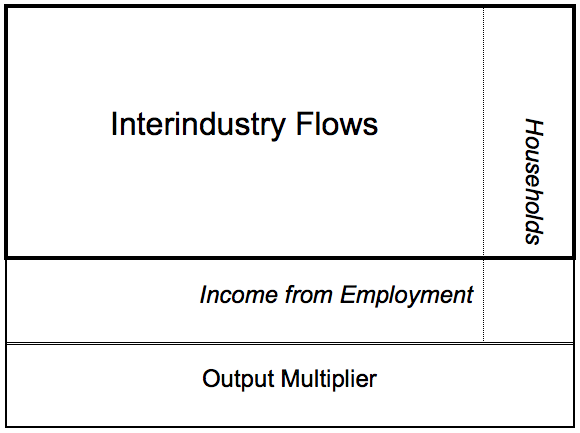
\includegraphics[width=3.5in]{T2OutputMultiplier}
  \caption{Type I Output Multiplier}
\end{figure}
\bigskip

The data used for the additional (Income from Employment) row for the Type II output multiplier (see Figure \ref{fig:4.3.2}), are wages. The IxI Tables give the ``Compensation of Employees'' for wages received. The corresponding total by which this row is divided in order to derive the $\textit{A}$-matrix entry for the Income from Employment row is the same as for the Interindustry flows. That is each sector's column total, the ``Total Output at basic prices''.

\bigskip

The second part for endogenising the Household sector is shown as the Households column in  Figure \ref{fig:4.3.2}. The cells used for this from the IxI Tables are the Household sectors ``Final Consumption Expenditure''. Note that this data is used in all the methods discussed in  Section \ref{sec:4.4}. The total used for the division of the Household cells for the A-matrix differs, however. Assessing which of these totals provides the best fit in comparison with the SAM multiplier is the motivation of this paper. For the purpose of illustration this paper uses the total from the Miller and Blair \citeA{Miller2009} method (see Section \ref{sec:4.4.1}). The total here for deriving the $a$-coefficients for the Household sector is the  ``Total Intermediate Demand'' of the ``Compensation of employees'' row at \textsterling63,560.9m \cite{ScottishGovernment2013a}.

\bigskip

Following the computation of the matrix of technical coefficients outlined above, the Leontief Inverse is computed. The method here is the same as for the Type I output multiplier in Section \ref{sec:4.3.1} (Equation \ref{eq:4.3.2} to \ref{eq:4.3.4}). The Leontief Inverse for the Type II is shown in Equation \ref{eq:4.3.5}.

  \bigskip  \begin{singlespacing}  \begin{equation} \label{eq:4.3.5}
  L=(I-A)^{-1} = Inverse   \begin{pmatrix}
  A_{II} &  A_{IH} \\
  A_{HI}  & A_{HH}
  \end{pmatrix} 
  \end{equation}   \end{singlespacing}  \bigskip

Equation \ref{eq:4.3.5} shows that the Leontief Inverse for the Type II multiplier now consists of additional technical coefficient entries in contrast to Equation \ref{eq:4.3.4}. These additions reflect the endogenised Household sector. $A_{II}$ is the technical coefficient matrix for the interindustry flows equal to Equation \ref{eq:4.3.1}. $A_{IH}$ is the amount of industry output required to satisfy Household demand. $A_{HI}$ is the amount of industry required per unit of total household income. $A_{HH}$ is household expenditure per unit of exogenous household income \cite{ScottishGovernment2013a}.

\bigskip

The computed value for the Agriculture-Agriculture entry for the Leontief Inverse differs to that of the Type I (see Section \ref{sec:4.3.1}). The Type I value is 1.156 and that for the Type II is 1.163 \footnote{ Note that this value differs depending on which method of the Type II output multiplier is used (see Section \ref{sec:4.3.1}).}. The Type II output multiplier is also bigger, as it is now 1.963, compared to 1.608 for the Type I. The following Section discusses the increase in multiplier value from Type I to Type II.

\subsubsection{Interpretation}

As noted above, the Type II output multiplier \footnote{ The Miller and Blair \citeA{Miller2009} method is used here for illustrative purposes (see Section \ref{sec:4.4.1}).} is larger than that of the Type I. This is due to the fact that the Type II multiplier models both the direct and indirect effects (like the Type I) as well as the induced effect. The induced effect results from the endogenising of the Household sector, as outlined in the Section above (see Section \ref{sec:4.3.2}).

\bigskip

Section \ref{sec:4.3.2})above outlined the direct effect and the indirect effect a demand shock of \textsterling1m in one sector. The induced effect observed in the Type II output multiplier results from additional household expenditure. The demand shock results in an output response throughout the economy (the direct- and indirect effects). It is assumed that the increase in output also has a positive effect on wages. Due to higher wages the Household sector increases expenditure and this is the induced effect.

\bigskip

Comparing the value of a Type I and a Type II output multiplier allows for the observation of the size of the induced effect. Following on from the example above, the Type II output multiplier (using the Miller and Blair \citeA{Miller2009} method introduced in Section \ref{sec:4.4.1}) below) is bigger by 0.355 \footnote{ The Type I output multiplier for Agriculture is computed at 1.608 and the Miller and Blair \citeA{Miller2009} Type II one at 1.963.}. Thus the initial \textsterling1m demand shock results in a multiplier effect in household expenditure of \textsterling355,000. Note that the size of the induced effect differs depending on which method of the Type II output multiplier is used.

\subsection{SAM Output Mulltiplier}
\label{sec:4.3.3}

The SAM output multiplier offers the most inclusive study of the multipliers discussed in this Section. As well as endogenising the Household sector, the SAM output multiplier also endogenises the Corporate sector. It uses a more comprehensive dataset and thus relies on more assumptions than the Type I or Type II output multiplier. Also note that the SAM output multiplier can only be computed in the presence of a suitable SAM.

\subsubsection{Calculation}

The basic calculation of the SAM output multiplier is very similar to the one outlined for the Type II in the Section above (see Section \ref{sec:4.3.2}). Figure \ref{fig:4.3.3}) shows which elements need to be added to the computation of the SAM output multiplier in order to endogenise the Corporate sector as well as the Household sector.

\bigskip
\begin{figure}[hb]
\label{fig:4.3.3}
  \centering
  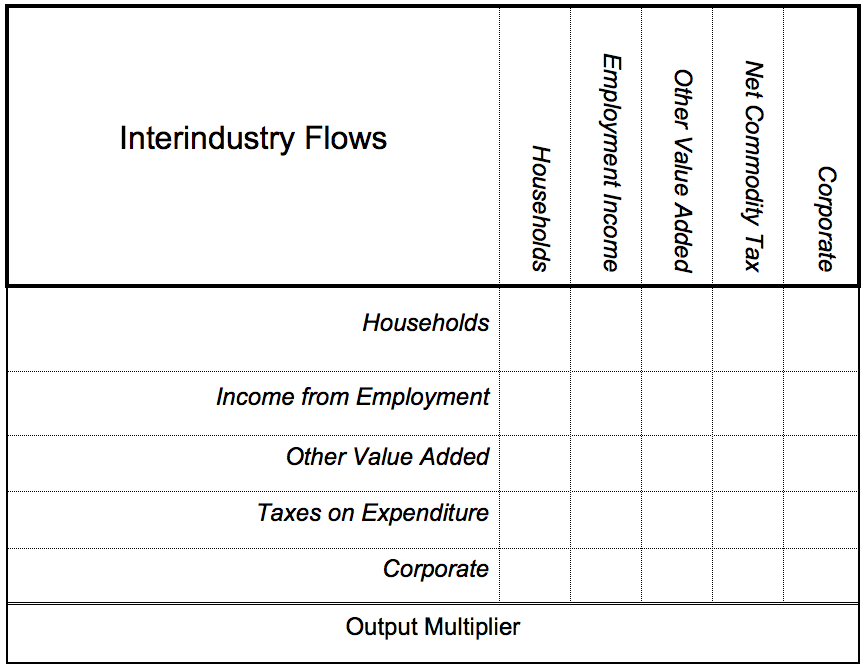
\includegraphics[width=4.5in]{SAMOutputMultiplier}
  \caption{Type I Output Multiplier}
\end{figure}
\bigskip

Equation \ref{eq:4.3.6} shows the Leontief Inverse of the SAM output multiplier. The interindustry matrix of technical coefficients is the $A_{II}$ in Equation \ref{eq:4.3.6}. The other data used for endogenising the Corporate Sector as well as the Household sector are shown as the additional row and column entries in Equation \ref{eq:4.3.6}. The interpretation of these vectors is equivalent to the added entries in Equation \ref{eq:4.3.5} (see Section \ref{sec:4.3.2}).

  \bigskip \begin{singlespacing}  \begin{equation} \label{eq:4.3.6}
  L=(I-A)^{-1} = Inverse   \begin{pmatrix}
  A_{II} & \cdots & A_{IC}  \\
  \vdots & \ddots & \vdots  \\
  A_{CI} & \cdots & A_{CC}
  \end{pmatrix} \end{equation} \end{singlespacing}  \bigskip

Note that the rows shown below the interindustry flows in Figure \ref{fig:4.3.3} are also not added to the multiplier figure (see Section \ref{sec:4.3.2} for comparison).

\subsubsection{Interpretation}

The interpretation of the SAM output multiplier follows along that of the Type II in Section \ref{sec:4.3.2}. The SAM multiplier computed here treats the Household- and the Corporate sector as endogenous.

\bigskip

... more

\bigskip

%%%%%%%%%%%%%%%%%%%%%%%%%%%%%%%%%%%%%%%%%%%%%%%%%%%%%%%%%%
%SECTION
%%%%%%%%%%%%%%%%%%%%%%%%%%%%%%%%%%%%%%%%%%%%%%%%%%%%%%%%%%

\newpage
    \section{Four Type II Methods}
\label{sec:4.4}

The previous Section outlined how the Type I, the Type II and the SAM output multiplier are computed. This basic structure for the derivation of these multipliers is used throughout the literature \textcolor{red}{REF} \footnote{ Additionally, there are various extensions for the Type II multiplier in particular \textcolor{red}{REF}, but this paper is concerned with the standard derivation of the Type II output multiplier.}. However, there are variations in what totals should be used for endogenising the Household sector in the Type II output multiplier as outlined in Section \ref{sec4.3.2}.

\bigskip

This Section outlines four methods used for the computation of the Type II output multiplier for Scotland. Section 5 analyses the results and compares the multipliers with each other. A benchmark value is needed in order to compare the different Type II multiplier methods. For this, it is assumed that the most complete set of accounts for the flow of goods and services in Scotland are given in a 2009 SAM for Scotland \cite{SCOSAM}. Thus, the SAM output multiplier is calculated and used as a benchmark \footnote{Note that a SAM multiplier automatically includes the Income from Employment and Household coefficients and thus is suitable to be used for a benchmark of the IO Type II's.}. The inter-industry flows as well as the Income from Employment and Household entries are the same for the IO and the SAM multiplier calculations. The variation of the multiplier values for the methods outlined below is due in part to the different Totals used for endogenising the Household sector. Thus the assumption is that the Totals closest in value to the Total used in the SAM multiplier calculations will derive the closest fitting multipliers.

\subsection{Miller and Blair}
\label{sec:4.4.1}

The first method analysed here originates from \citeA{Miller2009}, who use the total of the ``Compensation of Employee'' as the denominator for the technical coefficients of the Household sector \footnote{ Note, that this is the total of the Income from Employment row used by all four approaches.}. The corresponding value of this entry in the 2009 Scottish IxI Table is \textsterling63,561m \cite{ScottishGovernment2013a}.

\subsection{IxI Household Expenditure Total}
\label{sec:4.4.2}

The second method uses the ``Total Intermediate Consumption at basic prices'' of ``Households’ Final Consumption Expenditure''. This value is also given in the IxI Table and amounts to \textsterling65,421m \cite{ScottishGovernment2013a}.

\subsection{SAM Output Mulltiplier}
\label{sec:4.4.3}

The third method uses the total expenditure of the Household sector from the 2009 Scottish SAM \cite{SCOSAM}. This figure is derived by first, summing up the ``Final Consumption Expenditure'' of Households and ``Final Consumption Expenditure'' of Non-Profit Organisations Serving Households (NPISHs). Second, the Household expenditure on goods \& services of the following sectors are added to the Household Total: Rest of The World, Rest of the UK, Corporate, Government and Capital. This figure amounts to \textsterling107,877m.

\subsection{SAM Output Multiplier}
\label{sec:4.4.4}

The fourth method uses the combined Compensation of Employees at \textsterling63,561m from the IxI Table \footnote{ This is the Total used in the \citeA{Miller2009} method.} \cite{ScottishGovernment2013a} and all Unearned Income at \textsterling46,835m \cite{ScotGov2013c}. The total here is \textsterling110,396m. This figure is similar in nature to the one taken from the SAM above as it incorporates additional Household income sources. This is in contrast to the pure wage figures used, for example, in the \citeA{Miller2009} method. It is also the figure used for the official Scottish Government Leontief Inverse calculations.

\bigskip

Following on from the assumption placed above, the method using the Scottish SAM Household Total for endogenising the Household sector ought to be closest to the values derived by the SAM output multiplier. That is, the SAM uses the same Household Total for endogenising the Household sector. Next, the Combined Household Income Total is expected be closest. Then in descending order from Household Total value, the IxI Household Expenditure Total should give the third closest Type II estimate and lastly the one derived through the \citeA{Miller2009} method. However, it is worth noting that the Scottish SAM Household Total can only be used to derive the (IO) Type II if there is an applicable SAM. Hence the question arises whether pure IO modelling would allow for the presence of this type of IO multiplier.

%%%%%%%%%%%%%%%%%%%%%%%%%%%%%%%%%%%%%%%%%%%%%%%%%%%%%%%%%%
%SECTION
%%%%%%%%%%%%%%%%%%%%%%%%%%%%%%%%%%%%%%%%%%%%%%%%%%%%%%%%%%



%%%%%%%%%%%%%%%%%%%%%%%%%%%%%%%%%%%%%%%%%%%%%%%%%%%%%%%%%%%%%%%%%%%%%%%%%%%%%%%%%%%%%%%%%%%%%%%%%%%%%%%%%%%%%%%%%%%%%%%%%%%%%%%% SECTION 5
%%%%%%%%%%%%%%%%%%%%%%%%%%%%%%%%%%%%%%%%%%%%%%%%%%%%%%%%%%%%%%%%%%%%%%%%%%%%%%%%%%%%%%%%%%%%%%%%%%%%%%%%%%%%%%%%%%%%%%%%%%%%%%%%

\newpage
    \section{Results}
\label{sec:4.5}

This Section discusses the results of the multiplier computations. First, the raw multiplier values are discussed using descriptive analysis. Second, the different Type II output multipliers are compared to the SAM output multiplier using difference statistics. Third, error computations are utilized to determine a best fit of one of the four Type II output multipliers compared to the SAM output multiplier. Fourth, the results are summarized to provide a comprehensive overview of the findings in this Section.

\subsection{Multiplier Descriptives}
\label{sec:4.5.1}

Appendix A provides a full breakdown of the Type I, the Type II and the SAM output multipliers derived for 102 sectors of the 2009 Scottish IxI Tables and the 2009 Scottish SAM. This table allows for an in-depth analysis of the value of each multiplier for each sector. 

\bigskip

Furthermore, Appendix A shows the average values for each type of output multiplier. The Type I output multiplier is the lowest on average. This is to be expected, since this multiplier is computed using only the interindustry flow data from the IxI Tables. In contrast, the two largest average multiplier values are derived using the Miller and Blair and the IxI Household Expenditure Total methods (see Sections \ref{sec:4.4.1} and \ref{sec:4.4.2} ). Again this is to be expected, because these two methods use smaller values for the endogenising of the Household sector \footnote{The Miller and Blair value is \textsterling63,561m, and the IxI Household Expenditure Total value is \textsterling65,421m.}. In comparison, the other two methods outlined in Section \ref{sec:4.4} (see Sections \ref{sec:4.4.3} and \ref{sec:4.4.4}) use higher values for the endogenising of the Household sector \footnote{The Scottish SAM Household Total value is \textsterling107,877m, the Combined Household Income Total value is \textsterling110,396m.}. 

\bigskip

Using the SAM output multiplier as a benchmark, the average values show that the Miller and Blair as well as the IxI Household Expenditure Total method overestimate the average output multiplier effect. In contrast, the Scottish SAM Household Total and the Combined Household Income Total method underestimate the average output multiplier effect. Note though that the average difference of the latter compared to the SAM output multiplier is smaller. Lastly, Appendix A also shows the minimum and maximum multiplier values. These values reflect the analytics from above.


\bigskip
\begin{centering}
  \begin{table}[H]
\centering
  \caption{Descriptives Output Multiplier}
  \bigskip \begin{scriptsize}  \begin{doublespacing}
  \begin{tabular}{lrrrrrr}
  \toprule
   &  \begin{sideways}Type I\end{sideways} & \begin{sideways}Miller and Blair\end{sideways} & \begin{sideways}Scot Gov Stev\end{sideways} & \begin{sideways}Scot Gov SAM\end{sideways} & \begin{sideways}HH Exp\end{sideways} & \begin{sideways}SAM\end{sideways}   \bigstrut[b]\\
  \hline
           Average & 1.465 & 2.096 & 1.778 & 1.787 & 2.072 & 1.910 \\
           Minimum & 1.000 & 1.214 & 1.182 & 1.183 & 1.212 & 1.321 \\
           Maximum & 2.780 & 3.295 & 3.035 & 3.042 & 3.275 & 3.214 \\
  \hline \hline
      \end{tabular}%
        \bigskip  \label{tab:4.5.1}
      \end{doublespacing}  \end{scriptsize} \end{table}
      \end{centering}
\bigskip

\subsection{Multiplier Difference Statistics}
\label{sec:4.5.2}

Appendix B shows the differences between the Type II multiplier methods and the SAM benchmark. This allows for an in-depth study of which method of the multiplier is closest in value to the SAM multiplier broken down by individual sectors. This detailed analysis shows that there is not one method, which is closest in value for all sectors. For example, the first sector Agriculture shows that the Miller and Blair \cite{Miller2009} method gives the closest fitting multiplier at a value of 0.001\footnote{This value is calculated by taking the SAM multiplier value for the Agriculture sector of 1.964 and subtracting it by the relevant Miller and Blair method multiplier, which has a value of 1.963.}. For the same sector, the multiplier figure from the Combined Household Income Total shows the biggest difference at 0.180. In comparison, looking at the last sector, Households as Employers, using the SAM Household Income figure shows the smallest difference at 0.145. Here, the Miller and Blair \cite{Miller2009} version gives the biggest gap compared to the SAM at -0.485 with the Household Expenditure method following close behind at -0.435. This detailed analysis offers insights into which method might be offer the closest fit for different sectors. 

\bigskip

Note that the first two methods (Miller and Blair; IxI Household Expenditure Total) have mostly negative differences to the benchmark (see Appendix B)\footnote{Whilst the majority of sectors follow the same pattern, there are five sectors that diverge. Large differences between OVA and wages in those sectors seem to cause the reversed signs.}. In contrast, the last two methods described above (Scottish SAM Household Total; Combined Household Income Total) show only positive differences. These findings seem to suggest that the first two methods overestimate the Leontief Inverse. In contrast, the last two methods underestimate the Leontief Inverse compared to the benchmark. In order to be able to analyse which methods are closer to the benchmark, the absolute values of the differences in Appendix B are calculated (Appendix C).

\bigskip

The graph in Appendix C gives the ``Absolute Value Difference''\footnote{Absolute Value Differences - see word file}. The horizontal axis here can be interpreted to represent the SAM multiplier value and thus the closer the lines are to this axis, the better the fit. This graph shows that the two Type II methods using the more comprehensive household figure, the Scottish SAM Household Total and the Combined Household Income Total, give the closest fit to the SAM multiplier. The graph also strongly depicts that these two methods vary less in value compared to the first two Type II methods discussed above. The Miller and Blair \cite{Miller2009} method shows the overall biggest differences to the benchmark. In contrast, the Scottish SAM Household Total provides the closest fit in the graph. This confirms that endogenising the household sector using the SAM Household Total results in the closest fit.

\bigskip

Furthermore, Appendix C highlights that the difference between the methods varies substantially between the sectors. The methods using the Scottish SAM Household Total and the Combined Household Income Total for endogenising the Household sector show some variation compared to the benchmark. However, there are some very pronounced spikes observable in Appendix C for the Miller and Blair and the IxI Household Expenditure Total methods. The three biggest differences are for the Education (93), Security \& Investigation (89) and the Social Work (96) sectors. The multipliers for these sectors show large variation in comparison to the SAM output multiplier. These differences seem to be due to a small Gross Value Added to Total Output gap in the IxI Tables (REF).


\subsection{Error Computation}
\label{sec:4.5.3}

Table 1 shows various error-computations of the methods outlined above and the SAM benchmark. This allows for detailed measurements of the differences between the methods. The error-measurements in Table 1 are the ``Average of Differences''\footnote{This is the average of the differences for each sectoral multiplier derived from Appendix B.}, the Root Mean Squared Error (RMSE) and the Mean Absolute Error (MAE). The smallest value indicates the best fit with respect to the SAM output multiplier. All measurements show that endogenising the Household sector using the Scottish SAM Household Total figure results in the closest fit, followed by using the Combined Household Income Total figure. These two methods do not differ much in the error values. Also note that the values in Table 1 show that the four methods can be classified into two groups. First, the methods using pure IO data and second, the methods using the more comprehensive household expenditure figures. An example is the ``Average of Difference'' for Miller and Blair and the Household Expenditure total are estimated at 0.186 and 0.161, respectively. The same error computation for the Household Income from the SAM is given at 0.124 and that for the Household Income Scottish Government at 0.132.


\bigskip
\begin{centering}
  \begin{table}[H]
\centering
  \caption{RMSE and MAE Errors}
  \bigskip \begin{scriptsize}  \begin{doublespacing}
  \begin{tabular}{lrrrr}
  \toprule
  &  \begin{sideways}Miller and Blair\end{sideways} & \begin{sideways}Scot Gov Stev\end{sideways} & \begin{sideways}Scot Gov SAM\end{sideways} & \begin{sideways}HH Exp\end{sideways}   \bigstrut[b]\\
  \hline
  Average of Differences &  0.186 & 0.161 & 0.124 & 0.132   \\
  RMSE & 0.156 & 0.138 & 0.093 & 0.099   \\
  MAE & 0.101 & 0.089 & 0.065 & 0.070    \bigstrut[b]\\
  \hline \hline
  \multicolumn{5}{l}{Note: Smallest value shows closest fit to SAM multipliers}
      \end{tabular}%
        \bigskip  \label{tab:4.5.2}
      \end{doublespacing}  \end{scriptsize} \end{table}
      \end{centering}
\bigskip


The values in Table 1 also confirm that the Miller and Blair method results in the least close fit compared to the benchmark. In comparison, endogenising household expenditure using the IxI Household expenditure total, the Household sector column Total (2nd method from the left in Table 1) results in a closer fit. For example, the RMSE for the Miller and Blair method is given at 0.156 and the RMSE for the Household Expenditure total at 0.138. Therefore these results seem to suggest that computing a Type II with figures given only in the IO Tables would result in more accurate computations using the Household Expenditure total. 

\bigskip

The overall smallest error values are computed using the Scottish SAM Household Total. For example, is the MAE for this method is 0.065 and the next closest fit, the Combined Household Income Total, is 0.070. As noted above, the benchmark here is the SAM multiplier, due to the assumption that the 2009 Scottish SAM provides the most comprehensive single set of accounts of the Scottish economy for 2009. However, it is questionable whether pure IO modeling allows for the use of the SAM Household figure in endogenising household expenditure.

\subsection{Summary of Results}
\label{sec:4.5.4}

The general finding of this paper is that using more comprehensive household expenditure totals result in the closest fit of the Type IIs in comparison to the output multiplier derived from IxI data. An explanation for this is that not all household expenditure is covered using the income from employment figures from the Miller and Blair as well as the IxI Household Expenditure Total from the IxI Tables. Unearned income is part of households’ budgets and thus households’ total funds are bigger than those provided just in the IO Tables. Using these smaller income figures (Miller and Blair and IxI Household Expenditure Total) for endogenising household expenditure for the multiplier analysis is assumed to result in an overestimated Leontief Inverse. This in turn leads to a larger induced effect than is actually observed in the economy (REF IO Guide).

\bigskip

The findings in Appendix C confirm that using the first two methods result in overestimated figures of the Leontief Inverse. It must be noted, however, that the two methods using the more comprehensive Household Totals result in underestimated Leontief Inverses compared to the benchmark. Yet, the latter two methods observe smaller differences compared to the benchmark. 


%%%%%%%%%%%%%%%%%%%%%%%%%%%%%%%%%%%%%%%%%%%%%%%%%%%%%%%%%%%%%%%%%%%%%%%%%%%%%%%%%%%%%%%%%%%%%%%%%%%%%%%%%%%%%%%%%%%%%%%%%%%%%%%% SECTION 6
%%%%%%%%%%%%%%%%%%%%%%%%%%%%%%%%%%%%%%%%%%%%%%%%%%%%%%%%%%%%%%%%%%%%%%%%%%%%%%%%%%%%%%%%%%%%%%%%%%%%%%%%%%%%%%%%%%%%%%%%%%%%%%%%

\newpage
    \section{Conclusion}
\label{sec:4.6}

This paper shows that using the Total Household Income figure from the SAM for endogenising the Household sector results in the best multiplier fit. Note though that some of the other multiplier methods discussed above show closer fits for individual sectors. The overall best fit of the SAM Household Total method is to be expected since the SAM output multiplier is used as the benchmark. It is questionable, however, whether using a SAM entry for the derivation of an IO multiplier is theoretically correct. Similarly, using the Combined Household Income Total value for endogenising the Household sector relies on the availability of a data source exogenous to the IxI Tables. This paper finds that using the IxI Total Household Expenditure Total method is the best fit if the methods using exogenous data to the IxI Tables are not used. Thus, this paper has also shown that the widely used Miller and Blair method (REF) often derives the least best fitting Type II output multipliers. Thus, using the IxI Total Household Expenditure Total figure for the derivation of a pure IO Type II results in more accurate multipliers overall. 

\end{doublespacing}

\newpage
    \section{Appendix}
\label{sec:4.7}

\subsection{Appendix A}
\label{sec:4.7.1}
\bigskip
\textbf{Output Multiplier}

\begin{longtable}{@{\extracolsep{\fill}}rlrrrrrr@{}}
  &&  \begin{sideways}Type I\end{sideways} & \begin{sideways}Miller and Blair\end{sideways} & \begin{sideways}Scot Gov Stev\end{sideways} & \begin{sideways}Scot Gov SAM\end{sideways} & \begin{sideways}HH Exp\end{sideways} & \begin{sideways}SAM\end{sideways} \\ [0.5ex] 
    \hline 
    1     & Agriculture & 1.608 & 1.963 & 1.784 & 1.789 & 1.949 & 1.964 \\
    2     & Forestry planting & 1.615 & 2.069 & 1.840 & 1.846 & 2.051 & 1.972 \\
    3     & Forestry harvesting & 1.961 & 2.469 & 2.213 & 2.220 & 2.449 & 2.367 \\
    4     & Fishing & 1.611 & 1.962 & 1.785 & 1.790 & 1.949 & 1.933 \\
    5     & Aquaculture & 1.625 & 1.928 & 1.775 & 1.779 & 1.916 & 1.916 \\
    6     & Coal \& lignite & 1.671 & 2.079 & 1.874 & 1.879 & 2.063 & 1.983 \\
    8     & Other mining & 1.435 & 1.938 & 1.684 & 1.691 & 1.918 & 1.786 \\
    9     & Mining Support & 1.501 & 1.827 & 1.663 & 1.667 & 1.815 & 1.847 \\
    10    & Meat processing & 1.917 & 2.367 & 2.141 & 2.147 & 2.350 & 2.250 \\
    11    & Fish \& fruit processing & 1.695 & 2.184 & 1.937 & 1.944 & 2.165 & 2.044 \\
    12    & Dairy prod., oils \& fats processing & 1.923 & 2.430 & 2.174 & 2.181 & 2.410 & 2.300 \\
    13    & Grain milling \& starch & 1.803 & 2.257 & 2.028 & 2.035 & 2.240 & 2.134 \\
    14    & Bakery \& farinaceous & 1.426 & 2.031 & 1.726 & 1.735 & 2.007 & 1.840 \\
    15    & Other food & 1.609 & 2.139 & 1.872 & 1.879 & 2.118 & 1.980 \\
    16    & Animal feeds & 1.589 & 2.043 & 1.814 & 1.820 & 2.026 & 1.897 \\
    17    & Spirits \& wines & 1.299 & 1.738 & 1.516 & 1.523 & 1.721 & 1.694 \\
    18    & Beer \& malt & 1.367 & 1.775 & 1.570 & 1.575 & 1.760 & 1.746 \\
    19    & Soft Drinks & 1.493 & 2.009 & 1.749 & 1.756 & 1.989 & 1.872 \\
    21    & Textiles & 1.436 & 2.052 & 1.742 & 1.750 & 2.028 & 1.830 \\
    22    & Wearing apparel & 1.465 & 2.174 & 1.817 & 1.826 & 2.147 & 1.907 \\
    23    & Leather goods & 1.497 & 2.082 & 1.787 & 1.795 & 2.060 & 1.890 \\
    24    & Wood and wood products & 1.801 & 2.423 & 2.109 & 2.118 & 2.399 & 2.223 \\
    25    & Paper \& paper products & 1.662 & 2.163 & 1.911 & 1.918 & 2.144 & 2.010 \\
    26    & Printing and recording & 1.378 & 2.159 & 1.766 & 1.776 & 2.129 & 1.883 \\
    27    & Coke, petroleum \& petrochemicals & 1.204 & 1.302 & 1.253 & 1.254 & 1.299 & 1.321 \\
    28    & Paints, varnishes and inks etc & 1.421 & 1.924 & 1.671 & 1.678 & 1.905 & 1.756 \\
    29    & Cleaning \& toilet preparations & 1.460 & 2.139 & 1.797 & 1.806 & 2.113 & 1.895 \\
    30    & Other chemicals & 1.251 & 2.026 & 1.635 & 1.646 & 1.996 & 1.765 \\
    31    & Inorg. chem., dyestuffs \& agrochem. & 1.314 & 1.886 & 1.597 & 1.605 & 1.863 & 1.716 \\
    32    & Pharmaceuticals & 1.349 & 1.961 & 1.652 & 1.661 & 1.937 & 1.776 \\
    33    & Rubber \& Plastic & 1.491 & 2.199 & 1.843 & 1.852 & 2.172 & 1.948 \\
    34    & Cement lime \& plaster & 1.594 & 2.200 & 1.895 & 1.903 & 2.177 & 1.997 \\
    35    & Glass, clay \& stone etc & 1.473 & 2.144 & 1.806 & 1.815 & 2.118 & 1.915 \\
    36    & Iron \& Steel & 1.401 & 2.010 & 1.703 & 1.712 & 1.987 & 1.803 \\
    37    & Other metals \& casting & 1.449 & 1.982 & 1.713 & 1.721 & 1.962 & 1.831 \\
    38    & Fabricated metal & 1.481 & 2.185 & 1.830 & 1.840 & 2.157 & 1.941 \\
    39    & Computers, electronics \& opticals & 1.416 & 1.931 & 1.671 & 1.679 & 1.911 & 1.767 \\
    40    & Electrical equipment & 1.483 & 2.123 & 1.800 & 1.809 & 2.098 & 1.896 \\
    41    & Machinery \& equipment & 1.519 & 2.236 & 1.875 & 1.885 & 2.209 & 1.983 \\
    42    & Motor Vehicles & 1.515 & 2.121 & 1.816 & 1.824 & 2.098 & 1.907 \\
    43    & Other transport equipment & 1.647 & 2.211 & 1.927 & 1.935 & 2.190 & 2.026 \\
    44    & Furniture & 1.574 & 2.223 & 1.896 & 1.905 & 2.198 & 1.999 \\
    45    & Other manufacturing & 1.403 & 2.224 & 1.811 & 1.822 & 2.193 & 1.913 \\
    46    & Repair \& maintenance & 1.427 & 2.101 & 1.761 & 1.770 & 2.074 & 1.877 \\
    47    & Electricity & 2.053 & 2.375 & 2.213 & 2.217 & 2.363 & 2.345 \\
    48    & Gas etc & 1.260 & 1.519 & 1.389 & 1.392 & 1.509 & 1.482 \\
    49    & Water and sewerage & 1.287 & 1.694 & 1.489 & 1.495 & 1.679 & 1.708 \\
    50    & Waste & 1.493 & 2.135 & 1.811 & 1.820 & 2.110 & 1.941 \\
    51    & Remediation \& waste managem. & 2.780 & 3.295 & 3.035 & 3.042 & 3.275 & 3.214 \\
    52    & Construction - buildings & 1.766 & 2.347 & 2.054 & 2.062 & 2.324 & 2.200 \\
    53    & Construction - civil engineering & 1.731 & 2.388 & 2.057 & 2.066 & 2.363 & 2.202 \\
    54    & Construction - specialised & 1.530 & 2.223 & 1.874 & 1.883 & 2.196 & 2.020 \\
    55    & Wholesale \& Retail - vehicles & 1.335 & 2.049 & 1.689 & 1.699 & 2.021 & 1.815 \\
    56    & Wholesale - excl vehicles & 1.521 & 2.190 & 1.853 & 1.862 & 2.164 & 1.990 \\
    57    & Retail - excl vehicles & 1.352 & 2.071 & 1.709 & 1.719 & 2.044 & 1.858 \\
    58    & Rail transport & 1.764 & 2.512 & 2.135 & 2.145 & 2.483 & 2.265 \\
    59    & Other land transport & 1.400 & 1.979 & 1.687 & 1.695 & 1.956 & 1.810 \\
    60    & Water transport & 1.657 & 2.097 & 1.875 & 1.881 & 2.080 & 1.980 \\
    61    & Air transport & 1.467 & 1.881 & 1.672 & 1.678 & 1.865 & 1.792 \\
    62    & Support services for transport & 1.541 & 2.139 & 1.838 & 1.846 & 2.116 & 1.994 \\
    63    & Post \& courier & 1.278 & 2.259 & 1.765 & 1.778 & 2.221 & 1.893 \\
    64    & Accommodation & 1.352 & 2.004 & 1.675 & 1.684 & 1.979 & 1.814 \\
    65    & Food \& beverage services & 1.362 & 2.020 & 1.688 & 1.697 & 1.995 & 1.816 \\
    66    & Publishing services & 1.279 & 2.066 & 1.670 & 1.681 & 2.036 & 1.790 \\
    67    & Film video \& TV etc & 1.454 & 2.045 & 1.747 & 1.755 & 2.022 & 1.869 \\
    68    & Broadcasting & 1.386 & 1.987 & 1.684 & 1.692 & 1.963 & 1.819 \\
    69    & Telecommunications & 1.393 & 2.009 & 1.699 & 1.707 & 1.985 & 1.859 \\
    70    & Computer services & 1.250 & 2.041 & 1.642 & 1.653 & 2.010 & 1.789 \\
    71    & Information services & 1.185 & 1.918 & 1.549 & 1.559 & 1.890 & 1.719 \\
    72    & Financial services & 1.222 & 1.736 & 1.477 & 1.484 & 1.716 & 1.665 \\
    73    & Insurance \& pensions & 1.859 & 2.316 & 2.086 & 2.092 & 2.298 & 2.234 \\
    74    & Auxiliary financial services & 1.282 & 2.065 & 1.670 & 1.681 & 2.035 & 1.796 \\
    75    & Real estate - own & 1.465 & 1.742 & 1.603 & 1.606 & 1.732 & 1.817 \\
    76    & Imputed rent & 1.151 & 1.214 & 1.182 & 1.183 & 1.212 & 1.387 \\
    77    & Real estate - fee or contract & 1.503 & 2.139 & 1.818 & 1.827 & 2.114 & 1.971 \\
    78    & Legal activities & 1.241 & 1.998 & 1.617 & 1.627 & 1.969 & 1.781 \\
    79    & Accounting \& tax services & 1.202 & 2.040 & 1.617 & 1.629 & 2.007 & 1.786 \\
    80    & Head office \& consulting services & 1.391 & 2.192 & 1.789 & 1.800 & 2.161 & 1.914 \\
    81    & Architectural services etc & 1.437 & 2.171 & 1.801 & 1.811 & 2.142 & 1.953 \\
    82    & Research \& development & 1.423 & 2.439 & 1.927 & 1.941 & 2.400 & 2.057 \\
    83    & Advertising \& market research & 1.250 & 1.953 & 1.599 & 1.608 & 1.926 & 1.772 \\
    84    & Other professional services & 1.330 & 1.978 & 1.651 & 1.660 & 1.953 & 1.801 \\
    85    & Veterinary services & 1.364 & 2.126 & 1.742 & 1.752 & 2.096 & 1.918 \\
    86    & Rental and leasing services & 1.324 & 1.861 & 1.590 & 1.598 & 1.840 & 1.751 \\
    87    & Employment services & 1.301 & 2.261 & 1.778 & 1.791 & 2.224 & 1.918 \\
    88    & Travel \& related services & 1.520 & 1.900 & 1.709 & 1.714 & 1.886 & 1.786 \\
    89    & Security \& investigation & 1.155 & 2.273 & 1.709 & 1.725 & 2.229 & 1.853 \\
    90    & Building \& landscape services & 1.388 & 2.248 & 1.815 & 1.826 & 2.215 & 1.964 \\
    91    & Business support services & 1.285 & 1.925 & 1.602 & 1.611 & 1.900 & 1.769 \\
    92    & Public administration \& defence & 1.410 & 2.169 & 1.786 & 1.797 & 2.139 & 1.903 \\
    93    & Education & 1.189 & 2.367 & 1.774 & 1.790 & 2.322 & 1.914 \\
    94    & Health & 1.362 & 2.210 & 1.782 & 1.794 & 2.177 & 1.902 \\
    95    & Residential care & 1.320 & 2.243 & 1.778 & 1.791 & 2.207 & 1.950 \\
    96    & Social work & 1.236 & 2.388 & 1.807 & 1.823 & 2.343 & 1.959 \\
    97    & Creative services & 1.474 & 2.319 & 1.893 & 1.905 & 2.286 & 2.005 \\
    98    & Cultural services & 1.356 & 2.294 & 1.821 & 1.834 & 2.258 & 1.948 \\
    99    & Gambling & 1.414 & 1.888 & 1.649 & 1.656 & 1.870 & 1.822 \\
    100   & Sports \& recreation & 1.407 & 2.253 & 1.826 & 1.838 & 2.220 & 1.950 \\
    101   & Membership organisations & 1.436 & 2.253 & 1.841 & 1.852 & 2.221 & 1.970 \\
    102   & Repairs - personal and household & 1.357 & 2.055 & 1.703 & 1.713 & 2.028 & 1.822 \\
    103   & Other personal services & 1.233 & 1.886 & 1.557 & 1.566 & 1.861 & 1.732 \\
    104   & Households as employers & 1.000 & 2.284 & 1.637 & 1.655 & 2.234 & 1.799 \\
\hline
\caption{Output Multiplier}
\end{longtable}

\newpage

\subsection{Appendix B}
\label{sec:4.7.2}
\bigskip
\textbf{Differences Type II and SAM Output Multiplier}

\begin{longtable}{@{\extracolsep{\fill}}rlrrrr@{}}
  && \begin{sideways} Diff. Miller and Blair\end{sideways} & \begin{sideways} Diff. HH Expenditure IxI\end{sideways} & \begin{sideways} Diff. HH Income SAM\end{sideways} & \begin{sideways}Diff HH Income Scot Gov\end{sideways} \\ [0.5ex] 
    \hline 
    1     & Agriculture & 0.001 & 0.015 & 0.176 & 0.18 \\
    2     & Forestry planting & -0.097 & -0.079 & 0.126 & 0.132 \\
    3     & Forestry harvesting & -0.102 & -0.082 & 0.147 & 0.154 \\
    4     & Fishing & -0.029 & -0.015 & 0.143 & 0.148 \\
    5     & Aquaculture & -0.012 & 0     & 0.137 & 0.141 \\
    6     & Coal \& lignite & -0.096 & -0.081 & 0.104 & 0.109 \\
    8     & Other mining & -0.152 & -0.132 & 0.095 & 0.102 \\
    9     & Mining Support & 0.02  & 0.033 & 0.18  & 0.185 \\
    10    & Meat processing & -0.117 & -0.1  & 0.103 & 0.109 \\
    11    & Fish \& fruit processing & -0.14 & -0.121 & 0.1   & 0.107 \\
    12    & Dairy products, oils \& fats processing & -0.13 & -0.11 & 0.119 & 0.126 \\
    13    & Grain milling \& starch & -0.123 & -0.105 & 0.1   & 0.106 \\
    14    & Bakery \& farinaceous & -0.191 & -0.167 & 0.106 & 0.114 \\
    15    & Other food & -0.159 & -0.138 & 0.101 & 0.108 \\
    16    & Animal feeds & -0.147 & -0.129 & 0.076 & 0.083 \\
    17    & Spirits \& wines & -0.043 & -0.026 & 0.172 & 0.178 \\
    18    & Beer \& malt & -0.029 & -0.014 & 0.171 & 0.176 \\
    19    & Soft Drinks & -0.137 & -0.117 & 0.116 & 0.123 \\
    21    & Textiles & -0.222 & -0.198 & 0.08  & 0.088 \\
    22    & Wearing apparel & -0.267 & -0.24 & 0.08  & 0.09 \\
    23    & Leather goods & -0.193 & -0.17 & 0.095 & 0.103 \\
    24    & Wood and wood products & -0.2  & -0.176 & 0.105 & 0.114 \\
    25    & Paper \& paper products & -0.153 & -0.134 & 0.092 & 0.099 \\
    26    & Printing and recording & -0.275 & -0.245 & 0.107 & 0.118 \\
    27    & Coke, petroleum \& petrochemicals & 0.019 & 0.022 & 0.067 & 0.068 \\
    28    & Paints, varnishes and inks etc & -0.168 & -0.149 & 0.079 & 0.086 \\
    29    & Cleaning \& toilet preparations & -0.244 & -0.218 & 0.089 & 0.098 \\
    30    & Other chemicals & -0.261 & -0.231 & 0.119 & 0.13 \\
    31    & Inorganic chemic., dyest. \&agroch. & -0.17 & -0.147 & 0.111 & 0.119 \\
    32    & Pharmaceuticals & -0.185 & -0.161 & 0.115 & 0.124 \\
    33    & Rubber \& Plastic & -0.252 & -0.224 & 0.095 & 0.105 \\
    34    & Cement lime \& plaster & -0.203 & -0.18 & 0.094 & 0.103 \\
    35    & Glass, clay \& stone etc & -0.229 & -0.203 & 0.1   & 0.109 \\
    36    & Iron \& Steel & -0.207 & -0.183 & 0.091 & 0.1 \\
    37    & Other metals \& casting & -0.151 & -0.13 & 0.111 & 0.118 \\
    38    & Fabricated metal & -0.244 & -0.217 & 0.101 & 0.111 \\
    39    & Computers, electronics \& opticals & -0.164 & -0.144 & 0.089 & 0.096 \\
    40    & Electrical equipment & -0.227 & -0.202 & 0.087 & 0.095 \\
    41    & Machinery \& equipment & -0.254 & -0.226 & 0.098 & 0.108 \\
    42    & Motor Vehicles & -0.215 & -0.191 & 0.083 & 0.091 \\
    43    & Other transport equipment & -0.185 & -0.163 & 0.091 & 0.099 \\
    44    & Furniture & -0.224 & -0.198 & 0.095 & 0.104 \\
    45    & Other manufacturing & -0.311 & -0.28 & 0.091 & 0.102 \\
    46    & Repair \& maintenance & -0.224 & -0.198 & 0.106 & 0.115 \\
    47    & Electricity & -0.03 & -0.018 & 0.128 & 0.132 \\
    48    & Gas etc & -0.037 & -0.027 & 0.09  & 0.094 \\
    49    & Water and sewerage & 0.014 & 0.029 & 0.213 & 0.219 \\
    50    & Waste & -0.194 & -0.169 & 0.12  & 0.129 \\
    51    & Remediation \& waste management & -0.081 & -0.061 & 0.172 & 0.179 \\
    52    & Construction - buildings & -0.147 & -0.124 & 0.138 & 0.146 \\
    53    & Construction - civil engineering & -0.186 & -0.16 & 0.136 & 0.145 \\
    54    & Construction - specialised & -0.203 & -0.176 & 0.137 & 0.146 \\
    55    & Wholesale \& Retail - vehicles & -0.234 & -0.207 & 0.116 & 0.126 \\
    56    & Wholesale - excl vehicles & -0.2  & -0.174 & 0.128 & 0.137 \\
    57    & Retail - excl vehicles & -0.213 & -0.186 & 0.139 & 0.149 \\
    58    & Rail transport & -0.248 & -0.218 & 0.119 & 0.13 \\
    59    & Other land transport & -0.169 & -0.146 & 0.115 & 0.123 \\
    60    & Water transport & -0.118 & -0.1  & 0.098 & 0.104 \\
    61    & Air transport & -0.089 & -0.073 & 0.114 & 0.119 \\
    62    & Support services for transport & -0.145 & -0.122 & 0.148 & 0.156 \\
    63    & Post \& courier & -0.366 & -0.328 & 0.115 & 0.129 \\
    64    & Accommodation & -0.19 & -0.165 & 0.129 & 0.138 \\
    65    & Food \& beverage services & -0.204 & -0.179 & 0.119 & 0.128 \\
    66    & Publishing services & -0.277 & -0.246 & 0.109 & 0.12 \\
    67    & Film video \& TV etc & -0.175 & -0.152 & 0.114 & 0.122 \\
    68    & Broadcasting & -0.168 & -0.145 & 0.127 & 0.135 \\
    69    & Telecommunications & -0.15 & -0.126 & 0.152 & 0.161 \\
    70    & Computer services & -0.252 & -0.222 & 0.136 & 0.147 \\
    71    & Information services & -0.199 & -0.171 & 0.16  & 0.171 \\
    72    & Financial services & -0.071 & -0.051 & 0.181 & 0.189 \\
    73    & Insurance \& pensions & -0.082 & -0.064 & 0.142 & 0.148 \\
    74    & Auxiliary financial services & -0.269 & -0.239 & 0.114 & 0.125 \\
    75    & Real estate - own & 0.075 & 0.086 & 0.211 & 0.215 \\
    76    & Imputed rent & 0.173 & 0.175 & 0.204 & 0.205 \\
    77    & Real estate - fee or contract & -0.168 & -0.143 & 0.144 & 0.153 \\
    78    & Legal activities & -0.217 & -0.188 & 0.154 & 0.164 \\
    79    & Accounting \& tax services & -0.253 & -0.221 & 0.157 & 0.169 \\
    80    & Head office \& consulting services & -0.278 & -0.247 & 0.114 & 0.126 \\
    81    & Architectural services etc & -0.218 & -0.19 & 0.141 & 0.152 \\
    82    & Research \& development & -0.382 & -0.342 & 0.116 & 0.13 \\
    83    & Advertising \& market research & -0.181 & -0.154 & 0.163 & 0.173 \\
    84    & Other professional services & -0.177 & -0.152 & 0.141 & 0.15 \\
    85    & Veterinary services & -0.208 & -0.178 & 0.166 & 0.176 \\
    86    & Rental and leasing services & -0.11 & -0.089 & 0.154 & 0.161 \\
    87    & Employment services & -0.344 & -0.306 & 0.127 & 0.14 \\
    88    & Travel \& related services & -0.115 & -0.1  & 0.072 & 0.077 \\
    89    & Security \& investigation & -0.419 & -0.376 & 0.129 & 0.144 \\
    90    & Building \& landscape services & -0.284 & -0.25 & 0.138 & 0.15 \\
    91    & Business support services & -0.155 & -0.131 & 0.158 & 0.167 \\
    92    & Public administration \& defence & -0.266 & -0.236 & 0.106 & 0.116 \\
    93    & Education & -0.454 & -0.408 & 0.124 & 0.14 \\
    94    & Health & -0.308 & -0.275 & 0.108 & 0.12 \\
    95    & Residential care & -0.293 & -0.257 & 0.16  & 0.172 \\
    96    & Social work & -0.429 & -0.384 & 0.136 & 0.152 \\
    97    & Creative services & -0.314 & -0.281 & 0.101 & 0.112 \\
    98    & Cultural services & -0.347 & -0.31 & 0.113 & 0.126 \\
    99    & Gambling & -0.066 & -0.048 & 0.166 & 0.173 \\
    100   & Sports \& recreation & -0.303 & -0.27 & 0.111 & 0.123 \\
    101   & Membership organisations & -0.282 & -0.251 & 0.118 & 0.13 \\
    102   & Repairs - personal and household & -0.234 & -0.207 & 0.109 & 0.119 \\
    103   & Other personal services & -0.154 & -0.129 & 0.166 & 0.175 \\
    104   & Households as employers & -0.485 & -0.435 & 0.145 & 0.162 \\
\hline
\caption{Differences Type II and SAM Output Multiplier}
\end{longtable}

\newpage

\subsection{Appendix C}
\label{sec:4.7.3}

\begin{figure}[hb]
  \centering
  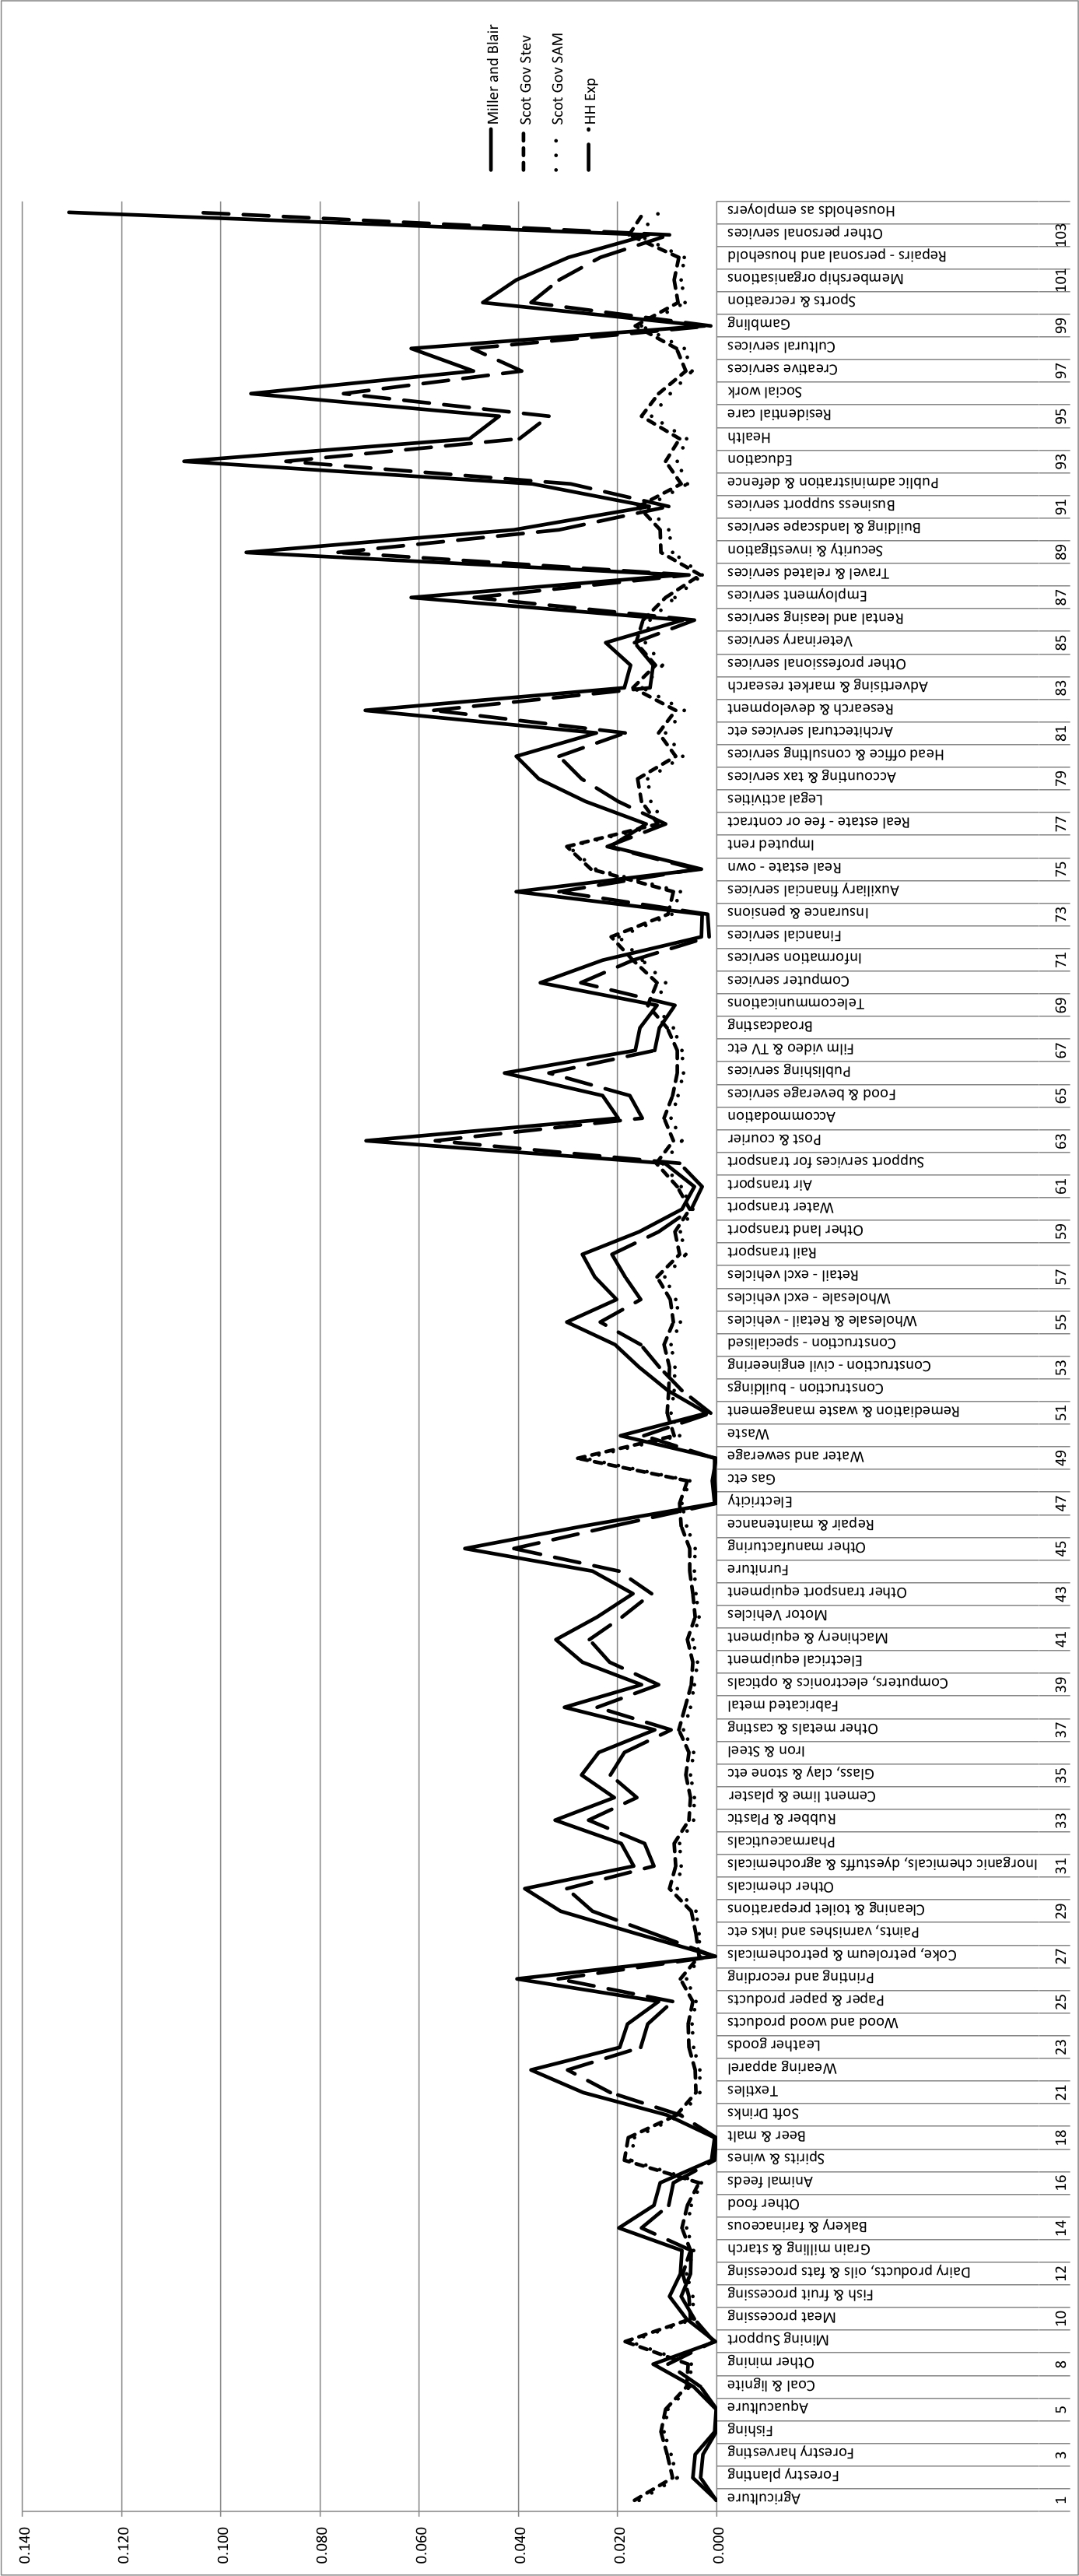
\includegraphics[width=3in]{DifferencesChart}
  \caption{Differences}
\end{figure}
